\pdfoutput=1
\documentclass[11pt]{article}
\usepackage[utf8]{inputenc}
\usepackage[T2A]{fontenc}
\usepackage[english,russian]{babel}
\usepackage{amsmath,amssymb,amsthm}
\usepackage[a4paper,left=24mm,right=20mm,top=22mm,bottom=24mm]{geometry}
\usepackage{graphicx}
\graphicspath{{../}}
\usepackage{array}
\usepackage{booktabs}
\usepackage{enumitem}
\usepackage[dvipsnames,table]{xcolor}
\usepackage{mdframed}
\usepackage[colorlinks=true,linkcolor=NavyBlue,citecolor=BrickRed,urlcolor=NavyBlue]{hyperref}

\newtheorem{theorem}{Теорема}
\newtheorem{lemma}{Лемма}
\newtheorem{proposition}{Предложение}
\newtheorem{corollary}{Следствие}
\theoremstyle{definition}
\newtheorem{definition}{Определение}
\theoremstyle{remark}
\newtheorem{remark}{Замечание}

\newcommand{\R}{\mathbb{R}}
\newcommand{\Z}{\mathbb{Z}}
\newcommand{\Q}{\mathbb{Q}}
\newcommand{\E}{\mathbb{E}}
\newcommand{\diam}{\operatorname{diam}}
\newcommand{\dist}{\operatorname{dist}}
\newcommand{\vol}{\operatorname{vol}}

% мягкая вёрстка: разрешить растяжку строк вместо выхода за поле
\setlength{\emergencystretch}{1.5em}

% рамка для ключевых утверждений
\newmdenv[linecolor=NavyBlue!60,linewidth=0.8pt,backgroundcolor=NavyBlue!4,
  roundcorner=4pt,skipabove=8pt,skipbelow=8pt,innertopmargin=6pt,
  innerbottommargin=6pt]{keybox}

% Статья 1 из комплекта (см. ../../journal/PLAN-2026-09-03-paper-split.md):
% только пять доказанных оценок. Статусные метки численных результатов и экранов здесь не вводятся.

\title{\bfseries Новые верхние оценки хроматических чисел
евклидовых пространств\\[2pt]
\large $\chi(\R^4)\le43$,\; $\chi(\R^5)\le132$,\; $\chi(\R^7)\le1029$,\;
$\chi(\R^9)\le7203$,\; $\chi(\R^{10})\le45619$%
\thanks{Код, точные сертификаты и данные открыты:
\url{https://github.com/ivaleo/Chromatic} (лицензия MIT).
Полная версия работы с поисковыми алгоритмами, лестницами ширин и
отрицательными экранами --- электронное дополнение \cite{Full}.}}
% Порядок авторов --- по вкладу (решение от 22.08.2026), не алфавитный.
\author{Л.\,Л.~Иванов\thanks{E-mail: \texttt{leo.ivanov@gmail.com}.}
  \and Н.\,В.~Глушкова\thanks{E-mail: \texttt{glushkova.nv@phystech.edu}.}}
\date{3 сентября 2026 г.}

\begin{document}
\maketitle

\begin{abstract}
\noindent
Раскраска евклидова пространства называется \emph{правильной для запрещённого
отрезка расстояний} $[1,\ell]$, если никакие две одноцветные точки не находятся
на расстоянии из $[1,\ell]$; наименьшее необходимое число цветов обозначается
$\chi\bigl(\R^n,[1,\ell]\bigr)$, а при $\ell=1$ это классическое хроматическое
число $\chi(\R^n)$ (проблема Нельсона--Хадвигера). Доказаны новые верхние
оценки
\[
\chi(\R^4)\le43,\quad \chi(\R^5)\le132,\quad \chi(\R^7)\le1029,\quad
\chi(\R^9)\le7203,\quad \chi(\R^{10})\le45619
\]
против известных $49$, $140$, $1372$, $17253$ и $3^{10}$; в частности,
опровергается ожидание Армана, Бондаренко, Прымака и Радченко, что $49$ и
$140$ минимальны среди всех решёточных раскрасок $\R^4$ и $\R^5$. Первые
четыре оценки даются явными рациональными решётками --- эйзенштейновой в
$\R^4$, общего положения в $\R^5$ и полученными ламинированием $E_6^*/343$ в
$\R^7$ и $E_8/2401$ в $\R^9$, --- а ключевое неравенство по единому протоколу
сведено к конечному списку неравенств между рациональными числами,
проверенных в точной арифметике. Последняя выводится аналитически из
продуктового правила для ширин $\sum_i1/d_i^2\le1$ и планарной нижней границы
$D((3+\omega)\Lambda)\ge\sqrt{7/3}\,\lambda_1$ для блока $E_8/2401$;
$45619$ --- первая оценка в $\R^{10}$ ниже классической башни $3^n$.
Код, точные сертификаты и данные открыты.
\end{abstract}

\begin{otherlanguage}{english}
\begin{center}
{\bfseries New upper bounds for the chromatic numbers of Euclidean spaces:\\
$\chi(\R^4)\le43$, $\chi(\R^5)\le132$, $\chi(\R^7)\le1029$,
$\chi(\R^9)\le7203$, $\chi(\R^{10})\le45619$}
\end{center}

\noindent\textbf{Abstract.}
A coloring of Euclidean space is proper for the forbidden distance segment
$[1,\ell]$ if no two points of the same color realize a distance in
$[1,\ell]$; the minimum number of colors is denoted $\chi(\R^n,[1,\ell])$,
and $\ell=1$ recovers the classical chromatic number $\chi(\R^n)$ of the
Nelson--Hadwiger problem. We prove the new upper bounds
$\chi(\R^4)\le43$, $\chi(\R^5)\le132$, $\chi(\R^7)\le1029$,
$\chi(\R^9)\le7203$, and $\chi(\R^{10})\le45619$, against the previously
known $49$, $140$, $1372$, $17253$, and $3^{10}$; in particular, this refutes
the expectation of Arman, Bondarenko, Prymak, and Radchenko that $49$ and
$140$ are optimal among all lattice colorings of $\R^4$ and $\R^5$. The
first four bounds come from explicit rational lattices --- an Eisenstein
lattice in $\R^4$, a lattice in general position in $\R^5$, and laminations
of $E_6^*/343$ in $\R^7$ and of $E_8/2401$ in $\R^9$ --- whose key inequality
is reduced, by a single verification protocol, to a finite list of
inequalities between rational numbers checked in exact arithmetic. The last
one follows analytically from a product rule for widths, $\sum_i1/d_i^2\le1$, and the planar lower bound
$D((3+\omega)\Lambda)\ge\sqrt{7/3}\,\lambda_1$ for the block $E_8/2401$;
$45619$ is the first bound in $\R^{10}$ below the classical $3^n$ tower.
All code, exact certificates, and data are open.

\smallskip
\noindent\emph{The paper is in Russian.}
\end{otherlanguage}

\section{Введение и основные результаты}\label{sec:intro}

\subsection{Задача}

\emph{Хроматическим числом плоскости} $\chi(\R^2)$ называется наименьшее число
цветов, в которые можно окрасить все точки плоскости так, чтобы никакие две
точки на расстоянии ровно~$1$ не оказались одного цвета. Этот вопрос, известный
как \emph{проблема Нельсона--Хадвигера} (ок.~$1950$), до сих пор не решён: с
$2018$~г. известно лишь $5\le\chi(\R^2)\le7$ \cite{deGrey,Soifer}. Аналогично
определяется $\chi(\R^n)$ для пространства любой размерности.

Естественное обобщение --- запрещать не одно расстояние, а целый \emph{отрезок}:
через $\chi\bigl(\R^n,[1,\ell]\bigr)$ обозначим наименьшее число цветов
раскраски, при которой одноцветные точки не реализуют ни одного расстояния из
отрезка $[1,\ell]$, $\ell\ge1$. При $\ell=1$ отрезок вырождается в точку и мы
возвращаемся к классическому $\chi(\R^n)=\chi\bigl(\R^n,[1,1]\bigr)$.
Систематическое изучение версии с интервалом начато первым автором
в~\cite{Ivanov2011}; в плоскости интервальная версия (в эквивалентной форме
запрета $[1-\varepsilon,1+\varepsilon]$) рассматривалась Экзоо
\cite{Exoo2005}; о современном состоянии плоского случая см.~\cite{ChJW}
и~\cite{Parts2023}. Поскольку запрет более широкого множества
расстояний требует не меньше цветов,
\begin{equation}\label{eq:mono}
\chi(\R^n)=\chi\bigl(\R^n,[1,1]\bigr)\ \le\ \chi\bigl(\R^n,[1,\ell]\bigr)
\qquad(\ell\ge1),
\end{equation}
и любая оценка сверху для интервальной версии автоматически оценивает
классическое хроматическое число. Подробнее об истории задачи см.
обзоры~\cite{BogolubskyRaigorodskii,Raigorodskii2001,Raigorodskii2013,Raigorodskii2014}.

Все известные \emph{верхние} оценки $\chi(\R^n)$ в малых размерностях получены
одним геометрическим приёмом --- \emph{периодической раскраской по разбиению
Вороного решётки} (\S\ref{sec:method}): пространство режется на ячейки Вороного
решётки $\Lambda$, и ячейка узла $v$ получает цвет класса смежности $v+\Gamma$
по подрешётке $\Gamma\subset\Lambda$ индекса $k$; раскраска правильна для
отрезка $[1,\ell]$, если \emph{нормированная ширина}
$d=D(\Gamma)/\diam V_0$ --- отношение наименьшего расстояния между
одноцветными ячейками к диаметру ячейки --- превосходит~$\ell$. Наилучшие
прежние значения в размерностях $4$--$10$ принадлежат Арману, Бондаренко,
Прымаку и Радченко~\cite{ABPR} (далее --- АБПР): $49$, $140$, $343$, $1372$,
$2401$, $17253$ и $3^{10}$.

Верхняя оценка в размерности~$4$ имеет историю: $\le54$ (Радоичич, Тот
\cite{RadoicicToth}, решётка $A_4^*$); оценка $\le49$ заявлена без
доказательства Кулсоном и приведена в \cite{CoulsonPayne2007}; полное
доказательство, вместе с проверкой минимальности индекса~$49$ \emph{для
решётки $D_4$}, дано в~\cite{ABPR}. Нижняя граница в этой размерности прошла
путь $6$ (Райский) $\to7$ \cite{Ivanov2006} $\to9$ \cite{ExooIsmailescu}.
В~\cite{ABPR} (открытый вопрос~1) высказана гипотеза, что улучшить $49$
нельзя:
\begin{quote}\itshape\small
<<We believe that the answer is negative for $n=4,5$, i.e.
$\min\chi_s(\E^4,\Lambda,\Lambda',\ell)=49$~\ldots>> (\cite{ABPR}, Open
question~1),
\end{quote}
где минимум берётся по всем решёткам $\Lambda$, подрешёткам $\Lambda'$ и всем
$\ell>0$. Настоящая работа опровергает эту гипотезу.

\subsection{Результаты}

\begin{keybox}
\begin{theorem}[сводная]\label{thm:summary}
\[
\chi(\R^4)\le43,\qquad \chi(\R^5)\le132,\qquad \chi(\R^7)\le1029,\qquad
\chi(\R^9)\le7203,\qquad \chi(\R^{10})\le45619 .
\]
Точнее, $\chi\bigl(\R^n,[1,\ell]\bigr)\le k$ при всех $\ell\le\ell_0$ для
пар $(n,k,\ell_0)$ из таблицы~\ref{tab:main}.
\end{theorem}
\end{keybox}

\begin{table}[htbp]\centering\small
\caption{Пять доказанных оценок. Столбец $\ell_0$ --- доказанная ширина
запрещённого отрезка $[1,\ell_0]$; запись $<x$ означает, что оценка доказана
при каждом $\ell<x$. Прежние оценки --- из~\cite{ABPR}. Каждая строка
проверяется одним маршрутом, указанным в последнем столбце
(таблица~\ref{tab:manifest} в \S\ref{sec:repro} даёт файлы и команды).}
\label{tab:main}
\begin{tabular}{@{}c r r l l l@{}}
\toprule
$n$ & было & стало & $\ell_0$ & доказательство & где \\
\midrule
$4$  & $49$    & $\mathbf{43}$    & $1{,}00411$      & точный рациональный сертификат & теорема~\ref{thm:main43}\\
$5$  & $140$   & $\mathbf{132}$   & $101/100$        & точный рациональный сертификат & теорема~\ref{thm:r5}\\
$7$  & $1372$  & $\mathbf{1029}$  & $103/100$        & точный рациональный сертификат & теорема~\ref{thm:r7ex}\\
$9$  & $17253$ & $\mathbf{7203}$  & $<1{,}0166127$   & точный рациональный сертификат & теорема~\ref{thm:r9ex}\\
$10$ & $3^{10}$& $\mathbf{45619}$ & $<\sqrt{217/214}$& аналитически (продуктовое правило) & теорема~\ref{thm:dim10}\\
\bottomrule
\end{tabular}
\end{table}

Доказательства устроены по двум схемам.

\emph{Явные конструкции с точными сертификатами} ($n=4,5,7,9$). В каждом случае
предъявляется рациональная матрица Грама $Q$ и целочисленная подрешётка, а
неравенство $d>\ell_0$ сводится к конечному списку неравенств между
рациональными числами, проверенных в точной арифметике дробей: точный
квадрат радиуса покрытия ячейки, доказуемо полный список опасных векторов и
для каждого из них сертификат Каруша--Куна--Таккера расстояния до ячейки.
Единый \emph{протокол} такой проверки сформулирован в \S\ref{sec:method}
(предложение~\ref{prop:protocol}), а четыре конструкции --- в
\S\ref{sec:constr}. Решётка индекса~$43$ \emph{эйзенштейнова}
($\Z[\omega]$-модуль ранга~$2$), решётка индекса~$132$ --- общего положения,
конструкции индексов~$1029$ и~$7203$ --- ламинирования эйзенштейновых
раскрасок $E_6^*/343$ и $E_8/2401$; плавающая точка участвует лишь в
\emph{выборе} кандидатов и активных множеств, но не в проверке.

\emph{Продуктовое исчисление ширин} ($n=10$). Для ортогонального
произведения раскрасок с ширинами $d_i$ условие правильности сворачивается в
одно неравенство $\sum_i1/d_i^2\le1$ (предложение~\ref{prop:product}), причём
блоки могут иметь разный индекс. Блок $E_8/2401$ имеет ширину не меньше
$\sqrt{7/6}$ --- это следует из \emph{оценки через проекцию на плоскость}
(предложение~\ref{prop:planar}: для любой эйзенштейновой решётки
$D((3+\omega)\Lambda)\ge\sqrt{7/3}\,\lambda_1$) и известного радиуса покрытия
$E_8$, --- и оставляет бюджет $1/7$; его хватает на плоский блок из
$19$ цветов ($6/7+4/31=214/217<1$, откуда $45619$ в~$\R^{10}$ --- первая
оценка в $\R^{10}$ ниже классической башни~$3^n$). Ни одного численного шага
в этом доказательстве нет (\S\ref{sec:product}). Тот же бюджет с одномерным
блоком из четырёх цветов даёт $\chi(\R^9)\le9604$ при
$\ell<\sqrt{63/61}$ (следствие~\ref{cor:dim9}); теперь эта оценка вытеснена
ламинированием: $7203$ цветов --- и при этом более широкий отрезок.

Все утверждения настоящей статьи --- теоремы или точные сертификаты.
Численные конструкции с меньшим числом цветов, лестницы ширин, эйзенштейново
тождество в полной форме, строгие экраны индекса и мозаичные раскраски вынесены
в сопутствующую статью~\cite{Widths}; поисковые алгоритмы, которыми конструкции
были найдены, отрицательные экраны и журналы кампаний --- в полную
версию~\cite{Full}. Раздел~\ref{sec:repro} содержит таблицу пяти утверждений с
входными данными, верификаторами и ожидаемым выводом.

\section{Критерий решёточной раскраски и протокол точной проверки}
\label{sec:method}

\subsection{Решётки, ячейки Вороного, раскраска классами смежности}

\emph{Решётка} $\Lambda\subset\R^n$ --- множество всех целочисленных линейных
комбинаций $n$ линейно независимых векторов $b_1,\dots,b_n$ (базиса).
\emph{Подрешётка} $\Gamma\subseteq\Lambda$ --- решётка, все узлы которой лежат
в $\Lambda$; её \emph{индекс} $k=[\Lambda:\Gamma]$ равен числу классов
смежности $\Lambda/\Gamma$ и вычисляется как модуль определителя
целочисленной матрицы перехода. \emph{Ячейкой Вороного} узла $a\in\Lambda$
называется множество точек, для которых $a$ --- ближайший узел:
\[
V_\Lambda(a)=\{x\in\R^n:\ \|x-a\|\le\|x-b\|\ \ \forall b\in\Lambda\}.
\]
Это выпуклый многогранник; все ячейки одинаковы с точностью до сдвига и
вместе замощают $\R^n$. Обозначим $V_0=V_\Lambda(0)$.

\begin{figure}[t]
\centering
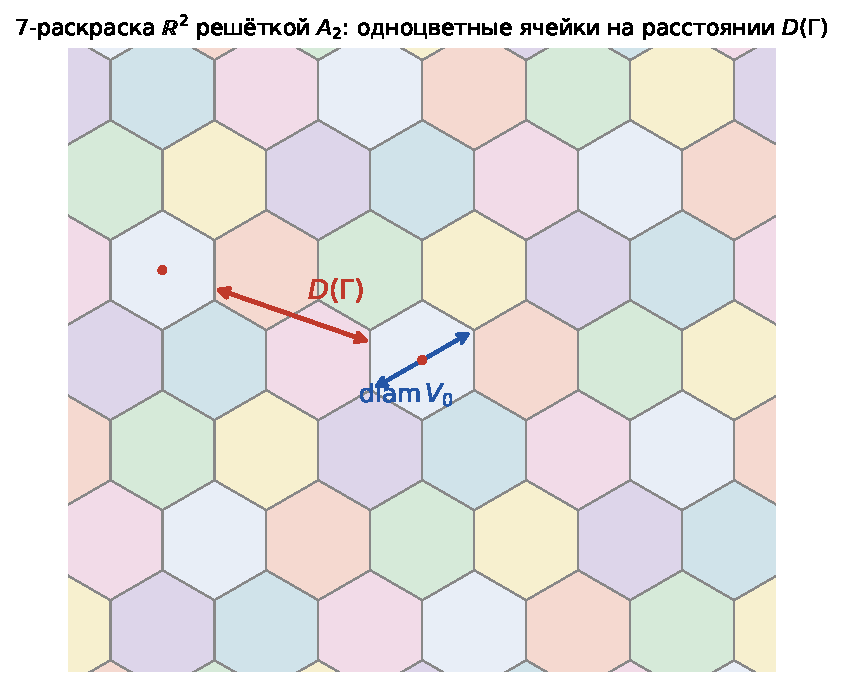
\includegraphics[width=0.62\textwidth]{fig_method.pdf}
\caption{Идея метода на примере $7$-раскраски плоскости шестиугольной решёткой
$A_2$ (конструкция Исбелла, $\chi(\R^2)\le7$). Каждая ячейка Вороного
окрашена цветом своего класса смежности по подрешётке индекса~$7$. Две
\emph{одноцветные} ячейки (красные точки) разделены расстоянием $D(\Gamma)$,
строго большим диаметра ячейки $\diam V_0$; раскраска запрещает все
расстояния из промежутка $\bigl(\diam V_0,\,D(\Gamma)\bigr)$.}
\label{fig:method}
\end{figure}

Зафиксируем подрешётку $\Gamma\subseteq\Lambda$ индекса $k$ и окрасим каждую
ячейку $V_\Lambda(v)$ цветом класса смежности $v+\Gamma$; получается
$k$-цветная периодическая раскраска $\R^n$ (рис.~\ref{fig:method}). Две точки
одного цвета лежат либо в одной ячейке, либо в ячейках $V_\Lambda(a)$,
$V_\Lambda(b)$ с $v=a-b\in\Gamma\setminus\{0\}$. В первом случае расстояние
не превосходит $\diam V_0$, во втором --- не меньше расстояния между
ячейками. Обозначим
\[
D(v)=\dist\bigl(V_0,\,v+V_0\bigr),\qquad
D(\Gamma)=\min_{v\in\Gamma\setminus\{0\}}D(v),\qquad
d(\Lambda,\Gamma)=\frac{D(\Gamma)}{\diam V_0}.
\]
Множество реализуемых одноцветных расстояний лежит в
$[0,\diam V_0]\cup[D(\Gamma),\infty)$, а открытый промежуток
$(\diam V_0,D(\Gamma))$ \emph{свободен}.

\begin{proposition}\label{prop:crit}
Если $d(\Lambda,\Gamma)>1$, то $\chi\bigl(\R^n,[1,\ell]\bigr)\le[\Lambda:\Gamma]$
при всех $\ell<d(\Lambda,\Gamma)$; в частности $\chi(\R^n)\le[\Lambda:\Gamma]$.
\end{proposition}
\begin{proof}
Возьмём масштаб $s>0$ с $s\,\diam V_0<1$ и $s\,D(\Gamma)>\ell$ --- это возможно
тогда и только тогда, когда $\ell<D(\Gamma)/\diam V_0=d$. Для решётки $s\Lambda$
свободный промежуток $\bigl(s\diam V_0,\,sD(\Gamma)\bigr)$ содержит весь отрезок
$[1,\ell]$, значит, раскраска правильна для $[1,\ell]$. Случай $\ell=1$ (с учётом
\eqref{eq:mono}) даёт $\chi(\R^n)\le k$.
\end{proof}

Величину $d$ называем \emph{нормированной шириной} запрещённого интервала.
Наименьшее число цветов среди раскрасок описанного вида принято обозначать
$\chi_s\bigl(\R^n,[1,\ell]\bigr)$; все известные верхние оценки в малых
размерностях, включая доказанные ниже, --- это оценки на $\chi_s$.

\begin{remark}[о границах ячеек]\label{rem:halfopen}
Ячейки Вороного замкнуты и пересекаются по границам, поэтому <<окрасим каждую
ячейку>> само по себе не задаёт функцию на $\R^n$. Как обычно, фиксируем
полуоткрытую фундаментальную область: из каждой пары соседних ячеек общая
грань приписывается одной из них. Оценки от этого выбора не зависят, так как
диаметр полуоткрытой ячейки не превосходит $\diam V_0$, а расстояние между
различными одноцветными ячейками не меньше $D(v)$.
\end{remark}

\subsection{Лемма о середине и окно полноты}

Ячейка $V_0$ --- выпуклый центрально-симметричный многогранник, и все её
фасеты центрально-симметричны (Вороной~\cite{Voronoi}); в частности
$\diam V_0=2R$, где $R=\max_{x\in V_0}\|x\|$ --- радиус покрытия. Центральная
симметрия сводит расстояние между двумя многогранниками к расстоянию от точки
до одного из них.

\begin{lemma}[о середине; {\cite[лемма~2]{Ivanov2011}}]\label{lem:mid}
Минимальное расстояние между $V_0$ и $v+V_0$ реализуется на паре точек,
симметричных относительно середины $v/2$ отрезка центров, поэтому
\begin{equation}\label{eq:mid}
D(v)=2\,\dist\bigl(v/2,\,V_0\bigr).
\end{equation}
\end{lemma}
\begin{proof}[Идея]
Пусть минимум достигается на $x\in V_0$, $y\in v+V_0$. Отражение относительно
$v/2$ переводит $V_0$ в $v+V_0$ и наоборот; образы $x',y'$ дают ту же длину.
Середины отрезков $[x,y']$ и $[y,x']$ по выпуклости лежат в соответствующих
ячейках, симметричны относительно $v/2$ и реализуют то же минимальное
расстояние; расстояние от каждой из них до $v/2$ равно $\dist(v/2,V_0)$.
\end{proof}

Минимум $D(\Gamma)$ берётся по бесконечной подрешётке, но перебирать нужно
конечное множество. Так как $V_0$ содержится в шаре радиуса $R=\frac12\diam V_0$,
справедливо $D(v)\ge\|v\|-\diam V_0$. Поэтому нарушить неравенство
$D(v)\ge\ell\diam V_0$ может лишь вектор с
\begin{equation}\label{eq:window}
\|v\|\ <\ (1+\ell)\diam V_0=2(1+\ell)R ,
\end{equation}
и это \emph{доказуемо полная} граница перебора: она не зависит от базиса
подрешётки. (Более узкое окно $\|v\|<4R$ отвечало бы лишь цели $d>1$ и для
интервального утверждения недостаточно.)

\subsection{Протокол точного сертификата}\label{ssec:protocol}

Три теоремы \S\ref{sec:constr} доказываются по одной схеме: численный
оптимум, найденный поиском (\cite[\S3]{Full}), округляется до рациональной
решётки, и дальше проверяется \emph{именно эта} решётка. Происхождение
кандидата на доказательство не влияет; влияет только приведённый ниже
конечный список проверок, каждая из которых выполняется в точной арифметике
дробей.

\begin{proposition}[протокол сертификата]\label{prop:protocol}
Пусть $Q\in\mathrm{Mat}_n(\Q)$ --- симметричная матрица с положительными
главными угловыми минорами, $\Lambda=\Z^n$ со скалярным произведением
$\langle x,y\rangle=x^{\mathsf T}Qy$, и $\Gamma=C\Z^n$ для целочисленной
$C$. Пусть конечная проверка установила:
\begin{enumerate}[leftmargin=2.2em,itemsep=1pt,label=\textup{(\roman*)}]
\item \emph{индекс}: $|\det C|=k$;
\item \emph{фасеты}: для каждого из $2^n-1$ ненулевых классов $\Lambda/2\Lambda$
найдены кратчайшие представители; классы с единственной парой $\pm v$
кратчайших дают список релевантных векторов $v$, и $V_0$ задаётся
неравенствами $\langle x,v\rangle\le\frac12\langle v,v\rangle$ по этому списку;
\item \emph{вершины}: перечислены все вершины $V_0$, причём полнота
доказана либо перебором всех $n$-подмножеств фасет, либо точным замыканием
по одномерному скелету; $R^2=\max\langle x,x\rangle$ по вершинам и
$\diam^2V_0=4R^2$;
\item \emph{окно}: перечислены все $v\in\Gamma\setminus\{0\}$ с
$\langle v,v\rangle<W$, где $W\ge\bigl(2(1+\ell_0)R\bigr)^2$ --- рациональная
граница;
\item \emph{разделение}: для каждого $v$ из окна предъявлены точка
$x^*\in V_0$ (допустимость проверена по всем фасетам) и множители
$\mu\ge0$ активных фасет с $v/2-x^*=\sum\mu_jv_j$, откуда
$D(v)^2=4\langle v/2-x^*,v/2-x^*\rangle$ точно;
\item \emph{запас}: $D_{\min}^2-\ell_0^2\,\diam^2V_0>0$ как рациональное число,
где $D_{\min}$ --- минимум по окну.
\end{enumerate}
Тогда $d(\Lambda,\Gamma)>\ell_0$ и $\chi\bigl(\R^n,[1,\ell]\bigr)\le k$ при
всех $\ell\le\ell_0$.
\end{proposition}

\begin{proof}
(ii)~--- теорема Вороного о релевантных векторах: $v$ задаёт фасету тогда и
только тогда, когда $\pm v$ --- единственная пара кратчайших представителей
класса $v+2\Lambda$; граница перебора внутри класса полна, поскольку у каждого
класса есть представитель с координатами из $\{0,1\}$, а кратчайший не длиннее
его. (iii)~--- максимум выпуклой функции $\langle x,x\rangle$ по многограннику
достигается в вершине; $\diam V_0=2R$ по центральной симметрии.
(iv)~--- окно~\eqref{eq:window}: вектор вне окна удовлетворяет
$D(v)\ge\|v\|-\diam V_0\ge\ell_0\diam V_0$ автоматически. (v)~--- условия
Каруша--Куна--Таккера достаточны для выпуклой задачи проекции на многогранник,
а по лемме~\ref{lem:mid} $D(v)=2\dist(v/2,V_0)$. (vi)~вместе с (iv), (v) даёт
$D(\Gamma)>\ell_0\diam V_0$, и остаётся предложение~\ref{prop:crit}.
\end{proof}

Дополнительный контроль, применяемый во всех сертификатах: центральная
симметрия множества вершин, соотношение Эйлера для $f$-вектора и равенство
$\vol V_0=\det\Lambda$. Плавающая точка используется лишь как
\emph{оракул-подсказчик} (перечислитель предлагает вершину, решатель --- активный
набор проекции); каждая принятая величина пересчитывается над $\Q$, поэтому
ошибка оракула может лишь остановить проверку, но не сделать её неверной.

\section{Точные конструкции в размерностях $4$, $5$, $7$ и $9$}
\label{sec:constr}

Каждая из четырёх теорем этого раздела предъявляет рациональную решётку и
подрешётку и доказывается протоколом предложения~\ref{prop:protocol}; ниже
приводятся данные конструкции и величины, которые протокол предъявляет.
Полные списки вершин, векторов окна и KKT-сертификатов лежат в файлах,
указанных в таблице~\ref{tab:manifest}. О том, как конструкции были найдены,
сказано по одному абзацу; подробности поиска --- в~\cite{Repo}.

\subsection{Размерность $4$: $\chi(\R^4)\le43$}\label{ssec:dim4}

\paragraph{Эйзенштейново семейство.}
Пусть $S\in\mathrm{GL}_4(\Z)$ --- элемент порядка~$3$ с характеристическим
многочленом $\Phi_3^2$ и $\Lambda$ --- решётка с $S\Lambda=\Lambda$. Тогда
$\Lambda$ --- $\Z[\omega]$-модуль ранга~$2$ ($\omega=e^{2\pi i/3}$), а
$S$-инвариантные положительно определённые формы образуют
четырёхпараметрическое семейство, определённое над~$\Q$: эрмитова форма
$h=\bigl(\begin{smallmatrix}a&c\\ \bar c&b\end{smallmatrix}\bigr)$ задаёт
вещественное произведение $\langle x,y\rangle=\operatorname{Re}h(x,y)$, и в
$\Z$-базисе $(e_1,\omega e_1,e_2,\omega e_2)$ её матрица Грама при
$u=\operatorname{Re}c$, $s=\tfrac{\sqrt3}{2}\operatorname{Im}c$ равна
\begin{equation}\label{eq:eisform}
Q(a,b,u,s)=\begin{pmatrix}
a & -\tfrac a2 & u & -\tfrac u2-s\\[2pt]
-\tfrac a2 & a & -\tfrac u2+s & u\\[2pt]
u & -\tfrac u2+s & b & -\tfrac b2\\[2pt]
-\tfrac u2-s & u & -\tfrac b2 & b
\end{pmatrix}.
\end{equation}
Если и подрешётка $S$-инвариантна, то она --- $\Z[\omega]$-подмодуль, и её
индекс есть норма идеала; $43=N(7+\omega)$ --- норма эйзенштейнова простого,
и подмодулей индекса~$43$ ровно $2\cdot44=88$. Сужение поиска до этого
семейства (три параметра вместо девяти, $88$ подрешёток вместо
$1+43+43^2+43^3=81\,400$) и дало конструкцию ниже; в полном пространстве форм
поиск останавливался ниже порога~\cite{Repo}.

\paragraph{Конструкция.}
Пусть $\Lambda_\star=B^{\mathsf T}\Z^4$, где $Q=BB^{\mathsf T}$ --- форма
\eqref{eq:eisform} с параметрами
\begin{equation}\label{eq:gram43}
a=1,\qquad b=\frac{39261}{25000},\qquad u=\frac{37381}{100000},\qquad
s=\frac{3141}{12500}
\qquad(200\,000\,Q\in\mathrm{Mat}_4(\Z)),
\end{equation}
и пусть $\Gamma_\star$ --- подрешётка индекса $43$ с матрицей перехода
(эрмитова нормальная форма; строки --- коэффициенты по базису $B$)
\begin{equation}\label{eq:hnf43}
T=\begin{pmatrix}1&0&0&41\\0&1&0&14\\0&0&1&37\\0&0&0&43\end{pmatrix},
\qquad\det T=43 .
\end{equation}
Инварианты (все рациональны, так как рациональна $Q$):
\[
\begin{aligned}
\lambda_1(\Lambda_\star)^2&=1,\\
\diam^2V_0&=\frac{5374343884337}{2019775849050}
  =2{,}660861544\ldots,\\
D(\Gamma_\star)^2&=\frac{7396075258066147}{2756867811550000}
  =2{,}682781969\ldots,
\end{aligned}
\qquad
\begin{aligned}
d(\Lambda_\star,\Gamma_\star)^2
&=\frac{298768283679964998359742207}{296327113258585430253847000}\\
&=1{,}008238093\ldots,\\
d&=1{,}004110598\ldots
\end{aligned}
\]
Ячейка $V_0$ имеет максимально возможные $30$ фасет и $f$-вектор
$(120,240,150,30)$. Решётка \emph{не} общего положения:
$\mathrm{Aut}(\Lambda_\star)\cong\Z/6$, три пары кратчайших векторов, и вся
группа автоморфизмов сохраняет $\Gamma_\star$, поэтому минимум $D$
достигается сразу на трёх парах $\pm v$ одной орбиты $\Z/3$.

\begin{keybox}
\begin{theorem}\label{thm:main43}
$\chi\bigl(\R^4,[1,\ell]\bigr)\le43$ при всех $1\le\ell\le\ell_0=1{,}00411$;
в частности, $\chi(\R^4)\le43$.
\end{theorem}
\end{keybox}

\begin{proof}[Доказательство --- протокол предложения~\ref{prop:protocol}]
\emph{Индекс:} $\det T=43$. \emph{Фасеты:} релевантные векторы --- минимумы
нормы в $15$ ненулевых классах $\Lambda_\star/2\Lambda_\star$, каждый класс
даёт единственную пару $\pm v$, итого $30$ фасет. \emph{Вершины:} решены все
$\binom{30}{4}=27\,405$ рациональных систем $4\times4$ с проверкой всех
неравенств; вершин ровно $120$, множество центрально симметрично,
$\vol V_0=\det\Lambda_\star$; отсюда $\diam^2V_0$ выше.
\emph{Окно}~\eqref{eq:window} при $\ell_0=1{,}00411$ перечислено полностью;
\emph{разделение:} для каждого вектора окна расстояние $\dist(v/2,V_0)$
вычислено точно --- активное множество берётся из плавающей точки, а
оптимальность подтверждается условиями Каруша--Куна--Таккера в дробях;
минимум $D^2$ выписан выше. \emph{Запас:}
\[
D(\Gamma_\star)^2-\ell_0^2\,\diam^2V_0
=\frac{3559631641205182621936510913}{1113651004958403329305500000000000}
=3{,}196\cdot10^{-6}>0 .
\qedhere
\]
\end{proof}

Независимой проверкой служит второй, \emph{опорный} сертификат: ячейка
заменяется объемлющим многогранником $P\supseteq V_0$ --- пересечением тех же
$30$ полупространств, --- для которого $\diam V_0\le\diam P$ и
$\dist(v/2,V_0)\ge\dist(v/2,P)\ge\bigl(\langle v/2,u\rangle-\max_{w\in
\mathrm{vert}P}\langle w,u\rangle\bigr)/\|u\|$ с рациональным направлением
$u$. Он даёт тот же диаметр (как дробь) и оценку снизу
$D(\Gamma_\star)^2\ge869307639027355969/324032161065600000=2{,}682781969\ldots$,
не превосходящую точного значения и превосходящую порог
$\ell_0^2\diam^2P=2{,}682778773\ldots$ Дополнительно исчерпывающим перебором
всех $81\,400$ подрешёток индекса~$43$ подтверждено, что~\eqref{eq:hnf43}
доставляет максимум $d$ для $\Lambda_\star$.

\begin{remark}[оптимум семейства]
Точка~\eqref{eq:gram43} --- рационализация (со знаменателем $10^5$) численного
оптимума задачи $\max d$ по трёхпараметрическому семейству; сам оптимум
устроен как жёсткое равноколебание (четыре $\Z/3$-орбиты векторов
$\Gamma_\star$ дают одно значение $D$, диаметр реализуется на $15$ парах
вершин) и численно равен $d=1{,}00411205721\ldots$ Исторически первой была
найдена другая решётка того же семейства с $200\,Q\in\mathrm{Mat}_4(\Z)$ и
$d^2=14984024/14873313$, $d=1{,}0037149\ldots$
(сертификат $\ell_0=1{,}003714$); именно её симметрия подсказала
семейство~\eqref{eq:eisform}.
\end{remark}

\subsection{Размерность $5$: $\chi(\R^5)\le132$}\label{ssec:dim5}

Прежняя оценка $140$ получена АБПР на решётке $A_5^*$, и там же доказана её
минимальность --- но лишь среди подрешёток \emph{этой} решётки. Конструкция
ниже найдена чередованием дискретного поиска ядра (подрешётка задаётся
сюръективным гомоморфизмом $\varphi\colon\Z^5\to\Z/132$) с непрерывной
деформацией формы Грама~\cite{Repo}; проверяется её
рационализация.

\begin{keybox}
\begin{theorem}\label{thm:r5}
$\chi\bigl(\R^5,[1,\ell]\bigr)\le132$ при всех $1\le\ell\le\dfrac{101}{100}$;
в частности, $\chi(\R^5)\le132$.
\end{theorem}
\end{keybox}

\begin{proof}[Доказательство --- протокол предложения~\ref{prop:protocol}]
Пусть $\Lambda=B^{\mathsf T}\Z^5$, где $BB^{\mathsf T}=Q$ и
\[
Q=\frac1{100000}
\begin{pmatrix}
79327&86284&69597&36140&26501\\
86284&254538&216808&101257&102135\\
69597&216808&296568&163667&140527\\
36140&101257&163667&181733&71653\\
26501&102135&140527&71653&148076
\end{pmatrix}.
\]
Её главные угловые миноры
\[
79327,\ 12746807270,\ 1422467480626358,\
124437401434750889345,\ 9999935596575703407615413
\]
положительны. Зададим цвет координатного вектора $x\in\Z^5$ тройкой
гомоморфизмов
\[
\begin{aligned}
\varphi_{11}(x)&=x_2+6x_3+2x_4+3x_5\pmod {11},\\
\varphi_3(x)&=x_1+2x_2+x_3\pmod 3,\\
\varphi_4(x)&=x_2+3x_3+x_4+3x_5\pmod 4.
\end{aligned}
\]
По китайской теореме об остатках это эквивалентно одной строке
\[
\varphi(x)=88x_1+89x_2+127x_3+57x_4+3x_5\pmod {132}.
\]
Положим $\Gamma=B^{\mathsf T}\ker\varphi$. Гомоморфизм сюръективен,
$[\Lambda:\Gamma]=132$, а диагональ Смита ядра равна $(1,1,1,1,132)$.

Ячейка Вороного рациональной формы $Q$ имеет $62$ фасеты и $720$ вершин.
Все вершинные системы решены над $\mathbb Q$; точный квадрат радиуса покрытия
равен
\[
R^2=
\frac{3093570095915736710467707313641}
     {3999974238630281363046165200000}.
\]
Доказываемое утверждение --- это $D(v)\ge\ell\,\diam V_0$ при $\ell=101/100$,
поэтому возможный нарушитель обязан удовлетворять
\begin{equation}\label{eq:win5}
\|v\|<2(1+\ell)R,\qquad\text{т.е.}\qquad \|v\|^2<12{,}4984\ldots
\end{equation}
Перебор Финке--Похста \cite{FinckePohst} по LLL-приведённому \cite{LLL}
базису $\Gamma$ оставляет в окне~\eqref{eq:win5} ровно $38$ ненулевых
векторов ($19$ пар); из них $36$ лежат уже в окне $\|v\|<4R$ и независимо
воспроизводятся C\raise.1ex\hbox{\small++}-перечислителем, а оставшаяся пара
$\pm(-2,2,-2,2,2)$ даёт $D/\diam V_0=1{,}0442\ldots$ и на минимум не влияет.

Для всех $38$ векторов задача проекции на $V_0$ решена точно: допустимость,
неотрицательность множителей KKT и значения целей проверены над $\mathbb Q$.
Минимум достигается на паре $\pm(2,0,1,-3,0)$ (координаты по базису
$\Lambda$) и равен
\[
\begin{aligned}
D_{\min}^2&=
\frac{1634114770527727}{516898614620000},\\
D_{\min}^2-\left(\frac{101}{100}\right)^2 4R^2
&=\frac{1450500657237822255902962097875907780124229}
{258447642807960215367421006872956903000000000}>0.
\end{aligned}
\]
Следовательно, $D_{\min}/\diam V_0=1{,}010897714548927\ldots>1{,}01$, и
раскраска ячеек по классам $\Lambda/\Gamma$ даёт требуемые $132$ цвета.
\end{proof}

Дополнительный верификатор, не использующий ни Qhull, ни вещественный
перечислитель коротких векторов, точно проверяет каждый из $31$ ненулевого
класса чётности, строит $62$ фасеты, обходит связный граф из $720$ вершин и
$1800$ рёбер и воспроизводит те же $R^2$, $D_{\min}^2$ и KKT-сертификаты.
Рационализация той же численной формы со знаменателями $10^4$ и $10^6$ даёт
отношения $1{,}010770760\ldots$ и $1{,}010904641\ldots$ --- в обоих случаях
строгий запас для $\ell=1{,}01$ сохраняется.

\subsection{Размерность $7$: $\chi(\R^7)\le1029$}\label{ssec:dim7}

\paragraph{Ламинирование.}
Базой служит эйзенштейнова раскраска $E_6^*/343$: $\Gamma'=(3+\omega)E_6^*$,
индекс $7^3=343$, ширина $\sqrt{7/6}$ (предложение~\ref{prop:planar} при
радиусе покрытия $E_6^*$, равном $\lambda_1/\sqrt2$~\cite{ConwaySloane}).
\emph{Ламинирование} строит раскраску $\R^7$ из раскраски $\R^6$: для
сдвига $c\in\R^6$, высоты $t>0$, склейки $a\in\Lambda'/\Gamma'$ и модуля
слоя $m$ положим
\[
\Lambda=\bigl\{(x+ic,\;it)\ :\ x\in\Lambda',\ i\in\Z\bigr\},\qquad
\Gamma=\bigl\{(x+ic,\;it)\ :\ \psi(x)+ia=0,\ m\mid i\bigr\},
\]
где $\Gamma'=\ker\psi$; тогда $[\Lambda:\Gamma]=343\,m$. При $m=3$ индекс
равен $1029$. Ячейка при подъёме растёт не более чем на $t^2$ по квадрату
диаметра, а расстояния между <<горизонтальными>> одноцветными ячейками не
убывают, так что запас ширины базы расходуется на высоту слоя; сдвиг $c$,
смещённый с орбит глубоких дыр $E_6^*$, и высота $t\approx1{,}08$ найдены
оптимизацией~\cite{Repo}. Проверяется рациональная точка: в
подходящем $\Z$-базисе семимерной решётки её матрица Грама и подрешётка
таковы:
% Сгенерировано из audit-data/results/dim7_1029_exact.json (не править вручную)
\begin{equation}\label{eq:gram1029}
\begingroup
\setlength{\arraycolsep}{3.2pt}
G=\begin{pmatrix}
30000&15000&0&-22500&15000&7500&-8632\\
15000&30000&22500&0&7500&15000&-4197\\
0&22500&45000&22500&0&22500&1601\\
-22500&0&22500&45000&-22500&0&6617\\
15000&7500&0&-22500&30000&15000&-5275\\
7500&15000&22500&0&15000&30000&4434\\
-8632&-4197&1601&6617&-5275&4434&17897
\end{pmatrix},\qquad Q=\frac{G}{10^{4}},
\endgroup
\end{equation}
\begin{equation}\label{eq:sub1029}
\begingroup
\setlength{\arraycolsep}{3.6pt}
C=\begin{pmatrix}
7&-5&0&0&0&0&0\\
0&1&0&0&0&0&0\\
0&0&7&-5&0&0&0\\
0&0&0&1&0&0&0\\
0&0&0&0&7&-5&0\\
0&0&0&0&0&1&0\\
0&0&0&0&0&0&3
\end{pmatrix},\qquad \det C=7^3\cdot3=1029 .
\endgroup
\end{equation}

Матрица $G$ имеет положительные главные угловые миноры; первые шесть базисных
векторов порождают базу, седьмой --- слоевой вектор $(c,t)$; три блока
$\bigl(\begin{smallmatrix}7&-5\\0&1\end{smallmatrix}\bigr)$ матрицы $C$
задают в трёх комплексных координатах базы идеал нормы~$7$ (умножение на
$3+\omega$ при подходящем выборе $\Z[\omega]$-структуры), множитель $3$ ---
модуль слоя; в частности, $D(\Gamma)$ достигается на образах минимальных
векторов базы.

\begin{keybox}
\begin{theorem}[точный сертификат в $\R^7$]\label{thm:r7ex}
Пусть $\Lambda=\Z^7$ со скалярным произведением $x^{\mathsf T}Qy$,
$Q=G/10^4$ из~\eqref{eq:gram1029}, и $\Gamma=C\Z^7$ с $C$
из~\eqref{eq:sub1029}, $\det C=1029$. Тогда
\[
D(\Gamma)^2=7,\qquad
\diam^2 V_0=\frac{96858928789031597}{14761819462500000},\qquad
d^2=\frac{103332736237500000}{96858928789031597},
\]
то есть $d=1{,}032878\ldots$, и $\chi\bigl(\R^7,[1,\ell]\bigr)\le1029$ при
всех $1\le\ell\le\dfrac{103}{100}$; в частности, $\chi(\R^7)\le1029$.
\end{theorem}
\end{keybox}

\begin{proof}[Доказательство --- протокол предложения~\ref{prop:protocol}]
\emph{Ячейка.} Релевантные векторы находятся по теореме Вороного о
$\Lambda/2\Lambda$; граница перебора $\max_{s\in\{0,1\}^7}Q(s,s)$ полна,
поскольку у каждого класса есть представитель из нулей и единиц; из
$300\,368$ перебранных векторов получаются $127$ пар, то есть $254$ фасеты,
максимум, возможный в $\R^7$ (ни один класс не вырождается).

\emph{Вершины.} Qhull лишь \emph{предлагает} точки; каждая переводится в
точную рациональную вершину решением целочисленной системы по $7$
независимым активным фасетам, после чего полный активный набор
пересчитывается над $\Z$. Полнота доказывается точным замыканием по
$1$-скелету: у каждой вершины перебираются все $6$-подмножества активных
фасет, и если подмножество ранга~$6$ задаёт допустимый экстремальный луч
касательного конуса, то второй конец соответствующего ребра обязан лежать в
наборе; связность $1$-скелета выпуклого многогранника доказывает полноту.
Простота \emph{не} предполагается --- и это существенно: из $30\,368$ вершин
$1\,600$ имеют по девять активных фасет. Отсюда точное
$R^2=96858928789031597/59047277850000000$ и $\diam^2V_0=4R^2$.

\emph{Разделение.} Улучшить текущий рекорд $D_*$ может лишь вектор с
$\|v\|<D_{*}+\diam V_0$; чтобы остаться в рациональных числах, берётся
подстраховка $(a+b)^2\le2(a^2+b^2)$, то есть перебор
$\|v\|^2\le2\bigl(D_{*}^2+\diam^2 V_0\bigr)=
200191665026531597/7380909731250000$. В это окно попадают $74$ вектора
($37$ пар); для каждого $D(v)^2=4\dist(v/2,V_0)^2$ предъявляется точный
KKT-сертификат --- множители $\mu\ge0$ и допустимость проекции.

\emph{Минимум} равен $7$ ровно и достигается на $27$ парах $\pm v$
\emph{горизонтальных} векторов (нулевая слоевая координата) --- образах
$54$ минимальных векторов $E_6^*$: это в точности пол
$\sqrt{7/3}\,\lambda_1$ предложения~\ref{prop:planar} в нормировке
$\lambda_1(E_6^*)^2=3$. Ближайший слоевой вектор даёт
$D^2=478385948533/68336903600\approx7{,}000404$, то есть превосходит порог с
запасом $7{,}6\cdot10^{-5}$ по~$D$.

\emph{Запас.} Для $\ell=103/100$
\[
D(\Gamma)^2-\ell^2\diam^2 V_0
=\frac{5750986852163787427}{147618194625000000000}>0 .
\qedhere
\]
\end{proof}

\begin{remark}[независимая проверка]\label{rem:r7second}
Неравенство $\diam^2V_0<7=D(\Gamma)^2$, а с ним $\chi(\R^7)\le1029$,
получено и вторым путём, не разделяющим с теоремой~\ref{thm:r7ex} ни одной
вычислительной детали: слоёная структура решётки позволяет ограничить радиус
покрытия сверху максимумом явной выпуклой квадратики по вершинам кусков
общего измельчения двух сдвинутых разбиений Вороного \emph{базы}
$E_6^*$ ($167$ кусков, $103$ из них доказано пустыми), причём в
шестимерной базе и без построения семимерной ячейки; максимум равен
$103310189182571717/59047277850000000=1{,}7496\ldots<7/4$, откуда
$\diam^2V_0\le6{,}99847\ldots<7$. Оба вычисления --- целиком в дробях;
подробности --- \cite{Repo}, \cite{Widths}.
\end{remark}

\subsection{Размерность $9$: $\chi(\R^9)\le7203$}\label{ssec:dim9}

\paragraph{Ламинирование.}
Схема та же, что в \S\ref{ssec:dim7}, но базой служит эйзенштейнова раскраска
$E_8/2401$: $\Gamma'=(3+\omega)E_8$, индекс $7^4=2401$, ширина $\sqrt{7/6}$
(предложение~\ref{prop:planar} при радиусе покрытия $E_8$, равном
$\lambda_1/\sqrt2$~\cite{ConwaySloane}). При модуле слоя $m=3$ индекс равен
$2401\cdot3=7203$; высота $t\approx1{,}15$ и сдвиг $c$ найдены
оптимизацией~\cite{Repo}. Проверяется
рациональная точка с $t^2=8264707/6250000$:
% Сгенерировано из audit-data/results/dim9_7203_exact.json (не править вручную)
\begin{equation}\label{eq:gram7203}
\begingroup
\setlength{\arraycolsep}{2.4pt}
G=\begin{pmatrix}
30000&15000&15000&-15000&-15000&15000&15000&15000&3329\\
15000&30000&15000&0&-15000&15000&15000&15000&6390\\
15000&15000&30000&0&0&0&0&0&4411\\
-15000&0&0&30000&0&0&0&-15000&-611\\
-15000&-15000&0&0&30000&-15000&-15000&-15000&-3579\\
15000&15000&0&0&-15000&30000&15000&15000&5606\\
15000&15000&0&0&-15000&15000&30000&15000&4509\\
15000&15000&0&-15000&-15000&15000&15000&30000&8550\\
3329&6390&4411&-611&-3579&5606&4509&8550&17982
\end{pmatrix},\qquad Q=\frac{G}{10^{4}},
\endgroup
\end{equation}
\begin{equation}\label{eq:sub7203}
\begingroup
\setlength{\arraycolsep}{3.0pt}
C=\begin{pmatrix}
-5&-2&-9&-5&-3&-6&-10&-3&0\\
4&3&-4&-3&0&0&-3&0&0\\
0&0&9&5&3&3&8&3&0\\
0&0&-5&-2&0&-3&-4&0&0\\
0&0&-4&-3&0&-1&-3&-1&0\\
0&0&4&3&1&3&3&1&0\\
0&0&0&0&0&0&2&-3&0\\
0&0&0&0&0&0&1&2&0\\
0&0&0&0&0&0&0&0&3
\end{pmatrix},\qquad \det C=-7203 .
\endgroup
\end{equation}

Верхний блок $8\times8$ матрицы $G$ --- решётка $E_8$ в нормировке
$\lambda_1^2=3$ (его определитель равен $(3/2)^8=6561/256$), девятая строка
задаёт слоевой вектор $(c,t)$. Смитова форма матрицы $C$ равна
$\operatorname{diag}(1,1,1,1,1,7,7,7,21)$, то есть
$\Lambda/\Gamma\cong(\Z/7)^3\times\Z/21$: четыре характера $\bmod\,7$ базы
и модуль слоя $3$.

\paragraph{Где было препятствие.}
В отличие от $\R^7$, априорной границы здесь не хватает: для ламинации
$\diam^2V_0\le4R_{\text{базы}}^2+t^2=6+t^2$, что даёт лишь
$R^2\le1{,}8306>7/4$, тогда как порог $D(\Gamma)^2=7$ требует $R^2<7/4$.
Поэтому всё утверждение упирается в один список --- полный набор вершин
девятимерной ячейки. Его удаётся получить после точной унимодулярной замены
базиса: вершин $1\,654\,230$ --- в пятьдесят с лишним раз больше, чем
$30\,368$ в~$\R^7$.

\begin{keybox}
\begin{theorem}[точный сертификат в $\R^9$]\label{thm:r9ex}
Пусть $\Lambda=\Z^9$ со скалярным произведением $x^{\mathsf T}Qy$,
$Q=G/10^4$ из~\eqref{eq:gram7203}, и $\Gamma=C\Z^9$ с $C$
из~\eqref{eq:sub7203}, $|\det C|=7203$. Тогда
\[
D(\Gamma)^2=7,\qquad
\diam^2 V_0=\frac{1119552292542693}{165294140000000},\qquad
d^2=\frac{1157058980000000}{1119552292542693},
\]
то есть $d=1{,}0166127\ldots$, и $\chi\bigl(\R^9,[1,\ell]\bigr)\le7203$ при
всех $1\le\ell<d$; в частности, $\chi(\R^9)\le7203$.
\end{theorem}
\end{keybox}

\begin{proof}[Доказательство --- протокол предложения~\ref{prop:protocol}]
\emph{Ячейка.} Релевантный вектор удовлетворяет $\|v\|^2\le4R^2\le6+t^2$, что
в единицах $G$ даёт границу перебора $73\,223$; из $4504$ перебранных векторов
получаются $376$ пар, то есть $752$ фасеты (потолок в $\R^9$ равен
$2(2^9-1)=1022$: $135$ классов $\Lambda/2\Lambda$ вырождаются и фасеты не
дают). Список фасет в доверенную базу не входит: любой набор целых векторов
решётки задаёт полупространства, содержащие $V_0$, поэтому пропуск фасеты мог
бы лишь увеличить $\diam V_0$ и уменьшить $D(\Gamma)$, то есть ослабить
оценку. Контроль: независимый перебор по классам $\Lambda/2\Lambda$ вовсе без
априорной границы даёт тот же набор из $752$ фасет.

\emph{Вершины.} Как и в теореме~\ref{thm:r7ex}, Qhull лишь \emph{предлагает}
точки, каждая переводится в точную рациональную вершину решением
целочисленной системы по $9$ независимым активным фасетам, а полнота
доказывается точным замыканием по $1$-скелету. Простота \emph{не}
предполагается: из $1\,654\,230$ вершин $1\,649\,640$ простые, $4320$ имеют по
пятнадцать и $270$ --- по шестнадцать активных фасет. Отсюда точное
\[
R^2=\frac{1119552292542693}{661176560000000}=1{,}69327281\ldots<\frac74,
\qquad \diam^2V_0=4R^2 .
\]

\emph{Разделение.} Перебор с подстраховкой $(a+b)^2\le2(a^2+b^2)$, то есть
$\|v\|^2\le2\bigl(D_{*}^2+\diam^2V_0\bigr)=2276611272542693/82647070000000$,
оставляет в окне $280$ векторов ($140$ пар); для каждого предъявляется точный
KKT-сертификат расстояния $D(v)^2=4\dist(v/2,V_0)^2$.

\emph{Минимум} равен $7$ ровно и достигается на $240$ \emph{горизонтальных}
векторах ($120$ пар, нулевая слоевая координата): это в точности пол
$\sqrt{7/3}\,\lambda_1$ предложения~\ref{prop:planar} в нормировке
$\lambda_1(E_8)^2=3$. Ни один слоевой вектор порога не нарушает.

\emph{Запас.} При $\ell=1$
\[
D(\Gamma)^2-\ell^2\diam^2 V_0=\frac{37506687457307}{165294140000000}
=0{,}2269\ldots>0,
\]
а при $\ell=101/100$ он ещё равен
$150036863771988707/1652941400000000000>0$.
\qedhere
\end{proof}

\begin{remark}[что даёт эта строка]\label{rem:r9beats}
Оценка $7203$ вытесняет прежнюю $\chi(\R^9)\le9604$ следствия~\ref{cor:dim9}
сразу по обоим параметрам: цветов меньше, а доказанный отрезок шире
($1{,}0166127\ldots$ против $\sqrt{63/61}=1{,}0162612\ldots$). На оценки в
$\R^{10}$ и выше она не влияет: в них девятимерный блок не участвует.
\end{remark}

\section{Планарная граница и продуктовое исчисление ширин}
\label{sec:product}

Оценки в размерностях $9$ и $10$ получаются без единого численного шага: из
одного точного факта о блоке $E_8/2401$ и одного правила сложения ширин.

\subsection{Планарная граница для эйзенштейновых конструкций}

Решётка $\Lambda\subset\R^n$ \emph{эйзенштейнова} (имеет
$\Z[\omega]$-структуру, $\omega=e^{2\pi i/3}$), если на ней задано умножение
на $\omega$, действующее изометрией порядка~$3$ без неподвижных ненулевых
векторов; тогда $\Lambda$ --- $\Z[\omega]$-модуль, и для
$\alpha\in\Z[\omega]$ подрешётка $\alpha\Lambda$ имеет индекс $|\alpha|^n$.
Конструкции АБПР $7^{n/2}$ цветов в размерностях $n=4,6,8,24$ --- это
$\Gamma=(3+\omega)\Lambda$ ($|3+\omega|^2=7$) на $D_4$, $E_6^*$, $E_8$ и
решётке Лича~\cite{ABPR}.

\begin{proposition}[планарная нижняя граница]\label{prop:planar}
Пусть $\Lambda\subset\R^n$ --- эйзенштейнова решётка. Тогда для каждого
ненулевого $w\in\Lambda$
\[
D\bigl((3+\omega)w\bigr)\ \ge\ \sqrt{7/3}\,\|w\|,
\qquad\text{в частности}\qquad
D\bigl((3+\omega)\Lambda\bigr)\ \ge\ \sqrt{7/3}\,\lambda_1(\Lambda),
\]
где $\lambda_1$ --- длина кратчайшего ненулевого вектора.
\end{proposition}

\begin{proof}
Векторы $\pm w,\ \pm\omega w,\ \pm(1+\omega)w$ лежат в $\Lambda$ и имеют одну
норму $\|w\|$ (умножение на обратимые элементы $\Z[\omega]$ --- изометрия
плоскости $P=\mathrm{span}(w,\omega w)$). Соответствующие шесть полупространств
$\langle x,u\rangle\le\|u\|^2/2$ содержат $V_0$, а их нормали лежат в $P$,
поэтому ортопроекция $\pi_P(V_0)$ содержится в правильном шестиугольнике $H$ ---
ячейке Вороного решётки $\Z[\omega]w\cong A_2$ масштаба $\|w\|$ внутри $P$.
Точка $v/2=(3+\omega)w/2$ лежит в $P$, проекция $1$-липшицева, и
\[
\dist\bigl(v/2,\,V_0\bigr)\ \ge\ \dist_P\bigl(v/2,\,H\bigr)
=\sqrt{7/12}\,\|w\|:
\]
в координатах плоскости при $\|w\|=1$ точка $(3+\omega)/2=(5/4,\sqrt3/4)$
лежит в нормальном конусе вершины $(1/2,\,1/(2\sqrt3))$ шестиугольника с
фасетами на расстоянии $1/2$, и квадрат расстояния до неё равен
$9/16+1/48=7/12$. По лемме~\ref{lem:mid}
$D(v)=2\dist(v/2,V_0)\ge\sqrt{7/3}\,\|w\|$; всякий ненулевой вектор
$(3+\omega)\Lambda$ имеет вид $(3+\omega)w$ с $w\ne0$, и $\|w\|\ge\lambda_1$.
\end{proof}

Для блока $E_8/2401$ этого достаточно. Решётка $E_8$ эйзенштейнова \cite{ConwaySloane,ABPR}; при минимальной
норме $\lambda_1^2=2$ её радиус покрытия равен~$1$ \cite{ConwaySloane}, так
что $\diam V_0=2$.
В нормировке $\lambda_1^2=3$ получаем $\diam^2V_0=6$, а по
предложению~\ref{prop:planar} $D\bigl((3+\omega)E_8\bigr)\ge\sqrt7$. Итак,
\begin{equation}\label{eq:e8width}
d\bigl(E_8,(3+\omega)E_8\bigr)^2\ \ge\ \tfrac76,\qquad
\bigl[E_8:(3+\omega)E_8\bigr]=7^4=2401 .
\end{equation}
(На самом деле здесь равенство --- минимум достигается на образах минимальных
векторов, см.~\cite{Widths}; для оценок ниже нужна только нижняя граница.)

\subsection{Правило сложения ширин}

\begin{proposition}[продуктовое исчисление]\label{prop:product}
Пусть $\Lambda=\bigoplus_{i=1}^{s}\Lambda_i$ --- ортогональная прямая сумма
решёток $\Lambda_i\subset\R^{n_i}$, и $\Gamma=\bigoplus_i\Gamma_i$ с
$\Gamma_i\subseteq\Lambda_i$. Обозначим $d_i=D(\Gamma_i)/\diam V_0(\Lambda_i)$
и $k_i=[\Lambda_i:\Gamma_i]$. Тогда после независимого масштабирования блоков
раскраска по $\Gamma$ правильна для интервала $[1,\ell]$ при всех
\[
\ell<\Bigl(\sum_i 1/d_i^2\Bigr)^{-1/2};
\]
в частности, $\chi\bigl(\R^{n},[1,\ell]\bigr)\le\prod_i k_i$, $n=\sum_i n_i$,
как только $\sum_i 1/d_i^2\le1$. Оптимум достигается при
$\diam^2 V_0(\Lambda_i)\propto 1/d_i^2$.
\end{proposition}

\begin{proof}
Ячейка Вороного прямой суммы есть произведение ячеек, поэтому квадрат
диаметра $V_0(\Lambda)$ равен $\sum_i\diam^2 V_0(\Lambda_i)$. Далее, для
$v=(v_1,\dots,v_s)$
\[
\dist(v/2,V_0)^2=\sum_i\dist\bigl(v_i/2,V_0(\Lambda_i)\bigr)^2,
\qquad\text{то есть}\qquad D(v)^2=\sum_i D_i(v_i)^2 .
\]
Так как $D_i(0)=0$, минимум по
$\Gamma\setminus\{0\}$ достигается на векторе с единственной ненулевой
компонентой, и условие $D(\Gamma)\ge\ell\diam V_0$ распадается на
$s$ условий
\[
d_i^2\,s_i\ \ge\ \ell^2\sum_j s_j,\qquad s_i:=\diam^2 V_0(\Lambda_i).
\]
Блоки можно масштабировать независимо, поэтому положим $s_i=S/d_i^2$; тогда
каждое условие обращается в равенство при $\ell^2=S/\sum_j s_j
=\bigl(\sum_j 1/d_j^2\bigr)^{-1}$, и по предложению~\ref{prop:crit} раскраска
правильна при всех меньших $\ell$. Любой другой выбор $s_i$ даёт не большее
$\ell$: минимум по $i$ величины $d_i^2 s_i/\sum_j s_j$ максимизируется именно
при пропорциональности. Наконец, правая часть монотонна по каждому $d_i$,
поэтому вместо точных ширин достаточно нижних оценок.
\end{proof}

Ширина оказывается не отчётом о качестве раскраски, а \emph{расходуемым
ресурсом}: блок с шириной $d_i$ стоит $1/d_i^2$ единиц бюджета, равного~$1$.
Существенно, что блоки могут иметь \emph{разный индекс}: именно смесь дорогого
широкого блока с дешёвым узким и работает.

\subsection{Размерности $10$ и $9$}

\begin{keybox}
\begin{theorem}\label{thm:dim10}
$\displaystyle\chi\Bigl(\R^{10},\bigl[1,\ell\bigr]\Bigr)\ \le\ 2401\cdot19=45619$
при всех $\ell<\sqrt{217/214}$; в частности, $\chi(\R^{10})\le45619$.
\end{theorem}
\end{keybox}

\begin{proof}
Берём два блока.

\emph{Блок $E_8$.} $\Gamma_1=(3+\omega)E_8$, индекс $2401$; по~\eqref{eq:e8width}
$d_1^2\ge7/6$, цена блока $1/d_1^2\le6/7$.

\emph{Плоский блок.} $\Lambda_2=aA_2$ --- шестиугольная решётка,
$\Gamma_2=(5+2\omega)\,aA_2$, индекс $N(5+2\omega)=19$. В плоскости ячейка
Вороного \emph{и есть} шестиугольник, поэтому $D$ вычисляется точно: при
$a=1$ ближайшая к точке $(5+2\omega)/2=(2,\sqrt3/2)$ точка шестиугольника с
фасетами на расстоянии $1/2$ --- его вершина $(1/2,1/(2\sqrt3))$, квадрат
расстояния до неё равен $9/4+1/3=31/12$, а по всем векторам $(5+2\omega)w$,
$w\in A_2\setminus\{0\}$, минимум достигается при $\|w\|=1$. Отсюда
$D(\Gamma_2)=2a\sqrt{31/12}$, $\diam V_0=2a/\sqrt3$ и $d_2^2=31/4$, цена
$1/d_2^2=4/31$.

Сумма цен $6/7+4/31=214/217<1$, и предложение~\ref{prop:product} даёт
$\ell<\sqrt{217/214}$ при $\prod k_i=2401\cdot19=45619$.
\end{proof}

Прежняя оценка в этой размерности --- $3^{10}=59049$ \cite{ABPR}, так что
выигрыш составляет $22{,}7\%$, и $45619$ --- первая оценка в $\R^{10}$ ниже
классической башни $3^n$. Оптимальный масштаб плоского блока
$a=\sqrt7\big/\bigl(2\sqrt{31/12}\bigr)=0{,}8230549\ldots$; сквозная численная
проверка построенной десятимерной решётки (индекс ровно $45619$,
$d=1{,}006984951\ldots$, совпадение с $\sqrt{217/214}$ до $10^{-9}$) в
доказательстве не участвует и служит лишь контролем.

\begin{keybox}
\begin{corollary}\label{cor:dim9}
$\displaystyle\chi\Bigl(\R^9,\bigl[1,\ell\bigr]\Bigr)\ \le\ 2401\cdot4=9604$
при всех $\ell<\sqrt{63/61}$; в частности, $\chi(\R^9)\le9604$.
\end{corollary}
\end{keybox}

\begin{proof}
Первый блок --- тот же $E_8/2401$ с ценой не выше $6/7$. Второй --- одномерный:
$\Lambda_2=\Z$, $\Gamma_2=4\Z$, четыре цвета. Ячейка Вороного --- отрезок
длины~$1$, две ближайшие одноцветные ячейки суть $[-1/2,1/2]$ и $[7/2,9/2]$,
расстояние между ними равно~$3$, поэтому $d_2=3$ и цена $1/d_2^2=1/9$. Сумма
цен $6/7+1/9=61/63<1$, и предложение~\ref{prop:product} даёт
$\ell<\sqrt{63/61}=1{,}016261\ldots$ при $\prod k_i=2401\cdot4=9604$.
\end{proof}

Три цвета не проходят: там $d_2=2$, цена $1/4$, и $6/7+1/4=31/28>1$ ---
бюджет $1/7$, оставленный блоком $E_8/2401$, требует ровно $d_2\ge\sqrt7$.
Оценка улучшает $17253$ работы~\cite{ABPR} на $44\,\%$. Тот же счёт с блоком
$\Lambda_{24}/7^{12}$ (у решётки Лича также $\lambda_1^2=4$ при радиусе
покрытия $\sqrt2$, то есть та же ширина $\sqrt{7/6}$) даёт
$\chi(\R^{25})\le4\cdot7^{12}$ и $\chi(\R^{26})\le19\cdot7^{12}$ против
$3^{25}$ и $3^{26}$; подробности, а также численные конструкции с меньшим
числом цветов в $\R^9$ и $\R^{10}$, чьи сертификаты диаметра пока выполнены в
плавающей точке, --- в~\cite{Widths}.

\section{Воспроизводимость}\label{sec:repro}

Весь код, точные сертификаты и данные открыты:
\begin{center}
\url{https://github.com/ivaleo/Chromatic}\quad (лицензия MIT).
\end{center}
Для пяти утверждений таблицы~\ref{tab:main} достаточно одного маршрута
каждому (таблица~\ref{tab:manifest}); все пути --- относительно каталога
\path{audit-data/}, команды выполняются из него.
Единый запуск
\begin{center}
\texttt{python -m chromatic\_research.campaigns.verify\_main\_results}
\end{center}
пересчитывает итоговые неравенства всех пяти строк из опубликованных
дробей на чистой рациональной арифметике за доли секунды (уровень~1 ниже),
а с флагом \texttt{--full} запускает и полные верификаторы строк $4$, $5$,
$7$ и $9$ (последний перечисляет $1\,654\,230$ вершин и занимает несколько
часов).

\begin{table}[htbp]\centering\footnotesize
\caption{Пять утверждений: вход, верификатор, ожидаемый вывод, уровень
независимости. Уровни: 1~--- пересчёт итоговых неравенств из опубликованных
дробей; 2~--- другой алгоритм в том же пакете; 3~--- независимая реализация
без общих геометрических процедур; 4~--- аналитическое доказательство.
Файлы данных лежат в \texttt{results/}, верификаторы --- в
\texttt{chromatic\_research/campaigns/}, тесты --- в \texttt{tests/}.}
\label{tab:manifest}
\setlength{\tabcolsep}{4pt}
\renewcommand{\arraystretch}{1.15}
\begin{tabular}{@{}l >{\raggedright\arraybackslash}p{4.4cm} >{\raggedright\arraybackslash}p{4.2cm} >{\raggedright\arraybackslash}p{3.5cm} c@{}}
\toprule
утверждение & вход & верификатор & ожидаемый вывод & ур.\\
\midrule
$\chi(\R^4)\le43$ & \path{r4_k43_eisenstein_rational.json} & \path{dim4_k43_verify.py} & $d^2=\frac{298768\ldots}{296327\ldots}>\ell_0^2$ & 3\\
 & \path{cert43_eisenstein.json} & опорный сертификат & \texttt{ok}; $D^2_{\downarrow}\ge\ell_0^2\diam^2P$ & 2\\
$\chi(\R^5)\le132$ & \path{metric_deform_a5_132_refined_certificate.json} & \path{certificate_window_fix.py} & $38$ векторов окна, запас $>0$ & 2\\
 & \path{metric_deform_a5_132_refined_independent_exact_audit.json} & \path{verify_exact_voronoi.py} & те же $R^2$, $D_{\min}^2$ & 3\\
$\chi(\R^7)\le1029$ & \path{dim7_1029_exact.json} & \path{dim7_1029_exact.py} & $D_{\min}^2=7$; \texttt{interval\_valid} & 2\\
 & --- & \path{dim7_1029_layer_cert.py} & $\max\varphi<7/4$ & 3\\
$\chi(\R^9)\le7203$ & \path{dim9_7203_exact.json} & \path{dim9_7203_exact.py} & $D_{\min}^2=7$; \texttt{interval\_valid} & 2\\
 & следствие~\ref{cor:dim9} ($9604$) & \path{test_product_calculus.py} & $6/7+1/9=61/63<1$ & 4\\
$\chi(\R^{10})\le45619$ & параметры двух блоков & \path{test_product_calculus.py} & $6/7+4/31=214/217<1$ & 4\\
\bottomrule
\end{tabular}
\end{table}

Каждый сертификат самодостаточен: рациональная форма Грама, матрица
подрешётки, точный квадрат радиуса покрытия, полный список векторов окна и
KKT-сертификат проекции для каждого из них; проверить его может короткая
программа, не имеющая ничего общего с кодом, которым он получен. Уровень~3
для строк $4$, $5$ и $7$ означает независимость \emph{кода}: перепроверки
выполнены программами, написанными с нуля и не разделяющими с основным
конвейером геометрических процедур (для $1029$ второй путь --- слоёный
сертификат замечания~\ref{rem:r7second}), но не независимыми исполнителями в смысле слепой репликации. Неизменяемая версия: настоящий текст отвечает коммиту
репозитория, указанному в файле \path{paper/article1/README.md};
архив с DOI будет указан при подаче.

\paragraph{Вклад авторов и использование ИИ.}
Постановка задачи, метод и вычислительный конвейер, конструкция индекса
$132$, ламинирование, продуктовое исчисление с оценками $9604$ и $45619$ и
планарная граница --- Л.\,Л.~Иванов. Н.\,В.~Глушковой принадлежат решётка
индекса~$43$ (первая точка семейства~\eqref{eq:eisform}, подсказавшая
симметрийное сужение) и точные рациональные верификаторы ламинирований
$E_6^*/343$ и $E_8/2401$, переведшие $1029$ и $7203$ из численных результатов
в теоремы~\ref{thm:r7ex} и~\ref{thm:r9ex}; во втором случае решающей была
точная унимодулярная замена базиса, без которой перечисление вершин
девятимерной ячейки не доводится до конца. Симметрийное сужение поиска и
независимые перепроверки --- совместные. Постатейный учёт с датами и коммитами ведётся
в репозитории (\path{CONTRIBUTIONS.md}). Вычислительный конвейер, скрипты
кампаний и первоначальные редакции текста первого автора создавались с
систематическим использованием ИИ-ассистента (большие языковые модели
общего назначения в агентной оболочке; коммиты несут трейлеры
\texttt{Co-Authored-By}); постановки, направление поиска, критерии отбора и
итоговая проверка принадлежат авторам, и для проверяемости теорем
происхождение поискового кода несущественно: каждая из них сведена к
конечному списку неравенств между явно выписанными рациональными числами.
Ответственность за все утверждения несут авторы.

\section{Заключение}

Доказано
\[
\chi(\R^4)\le43,\qquad \chi(\R^5)\le132,\qquad \chi(\R^7)\le1029,\qquad
\chi(\R^9)\le9604,\qquad \chi(\R^{10})\le45619
\]
против прежних $49$, $140$, $1372$, $17253$ и $3^{10}$: три оценки --- явными
рациональными конструкциями с точными сертификатами по единому протоколу,
две --- продуктовым исчислением ширин над блоком $E_8/2401$. В частности,
опровергнуто ожидание~\cite{ABPR}, что $49$ и $140$ минимальны среди всех
решёточных раскрасок $\R^4$ и $\R^5$. Ширина запрещённого интервала как
ресурс, точные лестницы ширин, эйзенштейново тождество в полной форме,
строгие экраны индекса и границы метода изучаются в~\cite{Widths}.


\begin{thebibliography}{99}\small

\bibitem{ABPR} A.~Arman, A.~Bondarenko, A.~Prymak, D.~Radchenko,
\emph{Upper bounds on chromatic number of $\E^n$ in low dimensions},
Electron. J. Combin. \textbf{31} ($2024$), no.~2, \#P2.35; arXiv:$2112$.$13\,438$.

\bibitem{ChJW} J.~Chybowska-Sok\'o\l{}, K.~Junosza-Szaniawski, K.~W\c{e}sek,
\emph{Coloring distance graphs on the plane},
Discrete Math. \textbf{346} ($2023$), no.~7, 113441;
arXiv:$2201$.$04\,499$.

\bibitem{ConwaySloane} J.~H.~Conway, N.~J.~A.~Sloane,
\emph{Sphere Packings, Lattices and Groups}, 3rd ed., Springer, $1999$.

\bibitem{CoulsonPayne2007} D.~Coulson, M.~S.~Payne,
\emph{A dense distance 1 excluding set in $\R^3$},
Austral. Math. Soc. Gaz. \textbf{34} ($2007$), no.~2, 97--102.

\bibitem{deGrey} A.~D.~N.~J.~de~Grey,
\emph{The chromatic number of the plane is at least 5},
Geombinatorics \textbf{28} ($2018$), no.~1, 18--31.

\bibitem{Exoo2005} G.~Exoo,
\emph{$\varepsilon$-unit distance graphs},
Discrete Comput. Geom. \textbf{33} ($2005$), 117--123.

\bibitem{ExooIsmailescu} G.~Exoo, D.~Ismailescu, M.~Lim,
\emph{On the chromatic number of $\R^4$},
Discrete Comput. Geom. \textbf{52} ($2014$), no.~2, 416--423.

\bibitem{FinckePohst} U.~Fincke, M.~Pohst,
\emph{Improved methods for calculating vectors of short length in a lattice},
Math. Comp. \textbf{44} ($1985$), 463--471.

\bibitem{Ivanov2006} Л.~Л.~Иванов,
\emph{Оценка хроматического числа пространства $\R^4$},
УМН \textbf{61} ($2006$), №~5, 181--182.

\bibitem{Ivanov2011} Л.~Л.~Иванов,
\emph{О хроматических числах $\R^2$ и $\R^3$ с интервалами запрещённых
расстояний}, Вестник РУДН, сер. Матем. Информ. Физ. ($2011$), №~1, 14--29.

\bibitem{Full} Л.~Л.~Иванов, Н.~В.~Глушкова,
\emph{Новые верхние оценки хроматических чисел евклидовых пространств:
полная версия} (электронное дополнение к настоящей статье и к~\cite{Widths}),
$2026$, \url{https://github.com/ivaleo/Chromatic/tree/main/paper}.

\bibitem{Widths} Л.~Л.~Иванов, Н.~В.~Глушкова,
\emph{Ширина запрещённого интервала как ресурс: эйзенштейново тождество,
ламинирование, экраны индекса и мозаичные раскраски евклидовых пространств},
$2026$ (сопутствующая статья).

\bibitem{LLL} A.~K.~Lenstra, H.~W.~Lenstra, L.~Lov\'asz,
\emph{Factoring polynomials with rational coefficients},
Math. Ann. \textbf{261} ($1982$), 515--534.

\bibitem{Parts2023} J.~Parts,
\emph{More certainty in coloring the plane with a forbidden distance
interval},
Geombinatorics \textbf{32} ($2023$), no.~4, 159--185; arXiv:$2303$.$14\,722$.

\bibitem{RadoicicToth} R.~Radoi\v{c}i\'c, G.~T\'oth,
\emph{Note on the chromatic number of the space},
in: Discrete and Computational Geometry, Algorithms Combin. \textbf{25},
Springer, $2003$, 695--698.

\bibitem{Soifer} A.~Soifer,
\emph{The Mathematical Coloring Book}, Springer, New York, $2009$.

\bibitem{Voronoi} Г.~Ф.~Вороной,
\emph{Собрание сочинений}, т.~2, Изд-во АН УССР, Киев, $1952$.

\end{thebibliography}
\end{document}
